\chapter{Theoretical Background and Related Work}
This section outlines key findings of related work on gender bias in MT, with a focus on the English-German (EN-DE) language pair to build the theoretical knowledge base. The research aims are to (1) define the core concept of gender bias in MT, (2) establish the relevance of the topic by reviewing related work, (3) identify the research gap, and (4) justify technical design choices. 

\vspace{1cm} 
\begin{figure}[htb]
    \centering
    \scalebox{0.8}{\tikzstyle{startstop} = [rectangle, rounded corners, minimum width=3.5cm, minimum height=1cm, text centered, draw=black, fill=gray!20]
\tikzstyle{process} = [rectangle, minimum width=3.5cm, minimum height=1cm, text centered, draw=black, fill=blue!10]
\tikzstyle{arrow} = [thick,->,>=stealth]

\begin{tikzpicture}[node distance=1.7cm]

\node (start) [startstop] {Define Key Concepts};
\node (review) [process, below of=start] {Review Related Work};
\node (gaps) [process, below of=review] {Identify Research Gaps};
\node (position) [process, below of=gaps] {Position Thesis Contribution};
\node (tech) [startstop, below of=position] {Explain Technical Approach};

\draw [arrow] (start) -- (review);
\draw [arrow] (review) -- (gaps);
\draw [arrow] (gaps) -- (position);
\draw [arrow] (position) -- (tech);

\end{tikzpicture}
}
    \caption{Overview of Chapter 2 Structure.}
    \label{fig:workflow_theory}
\end{figure}
\vspace{1cm} 

% --------------------------------------------------------------------------------

\section{Definitions}
This section explains the key terms and concepts needed to understand gender bias in EN-DE MT. It defines important ideas like Natural Language Processing (NLP), MT, and gender bias. These concepts provide the background necessary to follow the thesis.

\subsection{Natural Language Processing vs. Machine Translation}
    \textbf{NLP} refers to the development of machine systems that can process and generate human language. The goal is to mimic and understand it as fluently as possible \parencite{smacchiaDoesAIReflect2024,ullmannGenderBiasMachine2022}. Common applications are chatbots, translation tools, speech recognition, and image captioning.

    \textbf{MT} is a direct application of NLP. It is used to automatically translate text from one language to another \parencite{linMachineTranslationAcademic2009}. MT systems have gone through several stages of development; earlier approaches like rule-based and statistical MT used manually defined grammar rules or pattern matching from large translation corpora \parencite{chakravarthiSurveyOrthographicInformation2021}. 

    Most modern systems like Google Translate and DeepL, use neural machine translation (NMT) \parencite{wuGooglesNeuralMachine2016,deeplHowDoesDeepL2021}. These systems are trained on large sets of translated texts. They learn to represent the meaning of whole sentences as mathematical structures and generate more fluent and accurate translations. Unlike earlier systems, they aim to consider the full context of a sentence, which helps reduce errors and improves the handling of ambiguous or idiomatic language. In this work, all MT systems mentioned or deployed are neural NMT systems.

\subsection{Bias in Society and its Manifestations}
\label{subsection:manifestations_of_gb}
    Bias refers to a tendency to favour or disadvantage certain individuals or groups based on preconceived ideas. It often comes from stereotypes, which are fixed and oversimplified ideas about a group. While stereotypes describe what people think others are like, bias affects how they are treated.

    There are many kinds of bias. It can be based on age, disability, gender, ethnicity, religion, or sexual orientation \parencite{ullmannGenderBiasMachine2022}. These forms of bias often come from cultural and historical beliefs about how people in these groups should behave. 

    This work focuses on gender bias. It is the most visible form of bias in MT due to how language works. Gendered words, job roles, and grammar patterns can all affect translations and often repeat stereotypes. 
    
    Drawing on key studies that examine gender bias in EN-DE MT \parencite{ullmannGenderBiasMachine2022,rescignoGenderBiasMachine2023,lardelliBuildingBridgesDataset2024,kapplAreAllSpanish2025}, such bias typically manifests in the following forms:

    \subsubsection{Defaulting to Masculine Forms}
        In both singular and plural contexts, the \textit{generic masculine} refers to the default use of the masculine grammatical gender.
        For example, the sentence "Die Studenten sind im Hörsaal" (translation: "The students are in the lecture hall") uses the masculine plural form to refer to a group of students regardless of their gender.

        It is commonly used in spoken German and other gendered languages \parencite{lardelliBuildingBridgesDataset2024,schmitzGermanAllProfessors2022}, although research has consistently shown that the generic masculine creates a male bias in mental representations, leading readers or listeners to think more of male than female examples \parencite{sczesnyCanGenderFairLanguage2016}. 

    \subsubsection{Reinforcement of Stereotypes}
        Gender bias is deeply rooted in traditional views of men’s and women’s roles at work and at home \parencite{godsilEffectsGenderRoles2016}. Even though many of these roles are outdated, they still shape how people judge others’ abilities and character. This can lead to correspondence bias, where people assume traits based on behavior or context. These ideas are reinforced by media like TV shows and advertisements, and they can also influence the way language is used and interpreted.

        One common result of this is stereotypical job associations. People often link roles like doctors or pilots with he/him pronouns, and roles like nurses or flight attendants with she/her pronouns \parencite{shresthaExploringGenderBiases2022}. \textcite{pratesAssessingGenderBias2019} rates et al. also found clear patterns in how gender is associated with certain traits. Adjectives like "shy," "happy," "kind," and "ashamed" are often linked to women, while words like "arrogant," "cruel," and "guilty" are more often linked to men. 

  
 \subsection{Gender Bias in Machine Translation} \label{subsection:definition_gb}
    In MT, there is no clear definition of what counts as gender biased, nor is there a standard way to decide which features in text indicate it \parencite{barclayInvestigatingMarkersDrivers2024a}.

    Because of that, this work uses a simple rule-based definition to decide when a translation is considered gender biased:
        \begin{itemize}
        \item A gender-ambiguous subject in the source text is translated with a gendered term, often defaulting to the generic masculine (e.g., doctor → Arzt) or reflecting stereotypical gender roles (e.g., nurse → Krankenschwester).
        \item A gendered subject in the source text is assigned an incorrect gender in the translation, leading to semantic inconsistency (e.g., my mother is an engineer → meine Mutter ist ein Ingenieur).
        \end{itemize}

    This does not mean that all other cases are truly "unbiased". I will refer to anything that does not fall under these two cases as "neutral". This includes, but is not limited to:

        \begin{itemize}
        \item Sentences with no gendered terms, like "The weather is nice".
        \item Accurate translations of gendered input, like "The woman is a coder" → "Die Frau ist eine Programmiererin".
        \item The use of gender-fair alternatives (see \autoref{subsection:german_gfl}).
        \end{itemize}

    \begin{table}[htb]
    \centering
    \begin{tabularx}{\linewidth}{X | X}
        \toprule
        \textbf{Biased Translation} & \textbf{Neutral/Fair Translation} \\
        \midrule
        Gender-ambiguous source is translated with a gendered term. & 
        Gender ambiguity is preserved in the translation. \\
        \addlinespace[0.5em]
        Gendered subject is assigned an incorrect gender. & 
        Gender in the translation matches the gendered subject. \\
        \addlinespace[0.5em]
        \multicolumn{1}{c|}{—} & 
        Use of gender-fair language alternatives (see \autoref{subsection:german_gfl}). \\
        \bottomrule
    \end{tabularx}
    \caption{Summary of gender bias scenarios in translation (original compilation).}
    \label{tab:overview_bias_neutral}
    \end{table}

    We can observe that the translation errors often stem from two main sources: Model Overamplification and Semantic Bias. Both phenomena interact with skewed training data to produce the biased outputs outlined in \autoref{tab:overview_bias_neutral}.

    Model Overamplification occurs during training when the system exaggerates patterns that already exist in its data. If a corpus frequently pairs cooking with women, the model may conclude that cooking is inherently a female activity. This overemphasis can then manifest as the introduction of a gendered term where none existed or as the misassignment of a subject’s gender \parencite{ullmannGenderBiasMachine2022,shahPredictiveBiasesNatural2020}.

    Semantic Bias arises from the associations the model learns between words and genders. When “he” co‑occurs more often with “doctor,” the model will default to the masculine form in translation. Such defaults lead directly to outputs that either introduce an unwarranted gender or assign the wrong gender, as captured in the first two bias criteria. 
    
    Both overamplification and semantic bias worsen when training data are imbalanced. Studies report a high frequency of masculine forms in parallel corpora. One analysis found that the German term for “male doctor” appears 38 times more often than its female counterpart. Female and non‑binary examples remain far less common in many datasets \parencite{ullmannGenderBiasMachine2022,stanczakSurveyGenderBias2021}.

    Finally, the sheer scale of modern MT training sets makes manual review impossible. When a model is trained on hundreds of billions of tokens, it may unknowingly absorb and replicate harmful or offensive content. This reinforces the patterns that lead to the biased translations, underlining the need for targeted mitigation strategies at both the data and model levels \parencite{ullmannGenderBiasMachine2022}.

% --------------------------------------------------------------------------------

\section{Related Works}

    \subsection{Literature Search Process}
        For the literature review I combined incremental and conceptual literature review methods, where each source led to the identification of next. Based on this progression, I identified key concepts and used them to organize and interpret the literature, aligning with a conceptual approach. The structure followed the qualitative Information Systems framework by \textcite{schryenWritingQualitativeLiterature2015} and was further informed by \textcite{shresthaExploringGenderBiases2022} and \textcite{savoldiDecadeGenderBias2025}, who both conducted systematic reviews on gender bias in ML and MT respectively. 

        \subsubsection{Search Sources and Tools}
        Sources were primarily searched on \href{https://scholar.google.com/}{Google Scholar} and \href{https://www.perplexity.ai/}{Perplexity}, which served as an additional search engine. Prompts and outputs from Perplexity have been saved and are included in the appendix. To organize and manage the collected sources, \href{https://www.zotero.org/}{Zotero} was used throughout the process.

        \subsubsection{Literature Review Framing}
        To answer the four research aims, I have defined the key concepts in \autoref{tab:key-concepts}. Key search terms consisted of \textit{gender bias}, \textit{machine translation}, \textit{AI}, \textit{machine learning}, \textit{German}, \textit{stereotypes}, and \textit{detection}, which were combined with \textit{AND/OR}. The focus was on literature published between 2019 and 2025 to maintain relevance and currency, while foundational and definitional works from earlier periods were selectively included. The initial search for the term \textit{gender bias in machine translation} returned over 18,000 results. Through my iterative selection process, this was narrowed down to 34 core sources.

        \renewcommand{\arraystretch}{1.3}
            \begin{table}[ht!]
            \centering
            \begin{tabularx}{\textwidth}{>{\raggedright\arraybackslash}p{6.5cm}X}
            \toprule
            \textbf{Key Concept} & \textbf{Description} \\
            \midrule

            Foundations of Gender Bias in Natural Language Processing & Traces early research that identified gender bias in language. Focuses on foundational studies that showed why the issue matters and how later work builds on these findings. \\

            Sources and Manifestations of Bias & Explains how stereotypes shape language and persist over time. Describes how societal bias enters training data, model design, and system feedback. Shows how bias appears in machine translation and everyday language. \\

            Linguistic Challenges in English-German Translations & Explores key grammatical differences between English and German that affect translation. Focuses on how the lack of gender in English and its presence in German can lead to biased outputs. \\

            Mitigation Strategies and Current Limitations & Reviews how current research tries to reduce gender bias in NLP. Highlights what these methods can and cannot do. Helps identify where a classification-based approach could fill gaps and improve bias detection in translations. \\
            \bottomrule
            \end{tabularx}
            \caption{Key concepts relevant to this thesis}
            \label{tab:key-concepts}
        \end{table}


        \subsubsection{Citation Tracking}
        Backward citation searching involved reviewing references cited by selected papers, prioritizing frequently cited and foundational works relevant to gender bias in MT. Forward citation searching used Google Scholar's "cited by" function to identify newer research citing those key papers. Filtering with specific terms (e.g., \textit{German} and \textit{machine translation}) was applied during forward search to maintain focus. Beyond these systematic methods, I also included supplementary sources when needed while writing. These consist of contextual references, statistics, or secondary citations that support specific points but were not part of the core conceptual or methodological framework. Supplementary sources were defined as materials identified outside the systematic search, such as papers found through backward citations or targeted queries for statistics and news, which provided support for subordinate arguments without being central to the study's theoretical or analytical structure.

        \subsubsection{Selection Criteria and Screening Process}\label{subsection:selection_criteria}
        Titles and abstracts were manually screened to select relevant studies. Inclusion required sources to specifically address gender bias in MT, provide examples or discussions of gender-related errors, or explain the significance of gender bias in this context. Sources also had to be available in full text without access restrictions. Exclusion criteria filtered out studies focusing on general NLP bias without a direct link to MT, non-gender biases, and highly technical papers lacking contribution to the general understanding of gender bias or that did not provide additional knowledge beyond what was already found in previously published papers. Full texts were reviewed after initial screening to confirm relevance and extract insights. Redundant sources not providing new perspectives aligned with the thesis goals were excluded.

    \subsection{Foundational studies}
        The existence of gender bias in MT is well-documented. First mentions of this issue date back to over a decade ago, having been recognized by a paper by \citeauthor{schiebingerScientificResearchMust2014} in 2014. Since then, there has been a general increase in research papers focusing on this topic, especially between 2019 and 2023 \parencite{savoldiDecadeGenderBias2025}. 

        \textcite{pratesAssessingGenderBias2019} conducted a large-scale study using Google Translate to translate sentences like "[Gender-neutral pronoun] is an engineer" from twelve gender-neutral languages into English. The results showed a strong bias toward male pronouns, especially in STEM occupations. This could not be explained by real-world labor statistics, pointing instead to imbalances in the system's training data. The study received wide media attention, leading \citeauthor{googleReducingGenderBias2018} to change their translation policy: Google Translate began showing both feminine and masculine forms for ambiguous inputs \parencite{googleReducingGenderBias2018} (see \autoref{fig:gt_prates_example}).

        Building on this, \textcite{stanovskyEvaluatingGenderBias2019} created \href{https://github.com/gabrielStanovsky/mt_gender}{WinoMT}, a benchmark for evaluating gender bias in English-to-multilingual translations. It focused on occupations in contexts designed to challenge stereotypes. The study found that systems were more accurate for stereotypical gender roles but struggled in non-stereotypical cases, confirming the trends observed by \citeauthor{pratesAssessingGenderBias2019}.
        Together, these studies helped spark the ongoing research interest in gender bias in MT.

    \subsection{Why the topic remains relevant }
        Gender bias in MT can lead to representational harm. This happens when certain genders are repeatedly shown in biased or limiting ways through language \parencite{stanczakSurveyGenderBias2021}. These patterns can then again, enter training data and influence MT systems, and reflect back into society. This creates a regressive feedback loop.

        \vspace{1cm} 
        \begin{figure}[htb]
            \centering
            \scalebox{0.8}{
\begin{tikzpicture}[
    box/.style={rectangle, draw, rounded corners, minimum width=2.5cm, minimum height=1.2cm, align=center, font=\small},
    arrow/.style={-Stealth, thick, shorten >=1pt, shorten <=1pt},
    label/.style={midway, font=\footnotesize\bfseries}
]

\node[box] (bias) {Gender Bias\\in Society};
\node[box, right=3.5cm of bias] (data) {Training Data};
\node[box, right=3.5cm of data] (mt) {MT System};
\node[box, below=2.5cm of mt] (output) {Biased\\Outputs};
\node[box, below=2.5cm of bias] (harm) {Representational\\Harm};

\draw[arrow] (bias) -- (data) node[label, above] {1. Reflects};
\draw[arrow] (data) -- (mt) node[label, above] {2. Trains};
\draw[arrow] (mt) -- (output) node[label, right=3mm, xshift=2mm] {3. Produces};  
\draw[arrow] (output) -- (harm) node[label, above] {4. Causes};
\draw[arrow] (harm) -- (bias) node[label, left=3mm, xshift=-2mm, yshift=1mm] {5. Reinforces}; 

\end{tikzpicture}
}
            \caption{Regressive feedback loop of gender bias in MT.}
            \label{fig:regressive_feedback_loop}
        \end{figure}
        \vspace{1cm} 

        The generic masculine in particular leads to inaccurate and unfair representations of gender in translated text. \textcite{rescignoGenderBiasMachine2023} observed a predominance of masculine forms in translation outputs (approximately 90\% in Google Translate and 85–88\% in DeepL for EN-IT and EN-DE), even when the original sentences contained relatively few masculine references. This shows that the bias is not minor but occurs quite heavily in those systems.

        It also contributes to the invisibility of women in male-dominated professions \parencite{kapplAreAllSpanish2025}. Studies show that biased language in machine-generated text, such as children’s stories or job ads, can influence how young people view themselves \parencite{soundararajanInvestigatingGenderBias2024,kapplAreAllSpanish2025}. It may shape their interests, hobbies, and career choices. This is especially visible in STEM fields \parencite{pratesAssessingGenderBias2019}, where stereotypes are more persistent. When job descriptions or mock interviews use gender-exclusive pronouns, women report feeling less belonging, lower motivation, and weaker identification with the role \parencite{godsilEffectsGenderRoles2016}. Many self-select out of applying, shrinking the female talent pool and reinforcing gender gaps in the workforce.

        Research also shows that using GFL like "she and he" or "one" can improve how women respond to job ads. It reduces stereotype threat and helps them engage more positively with opportunities \parencite{godsilEffectsGenderRoles2016}.

        Furthermore, a study by \textcite{savoldiWhatHarmQuantifying2024} measured how much effort people need to fix biased translations. They used metrics like the time it took to edit and how many edits were needed, based on human-targeted error rate. The results showed that fixing translations with feminine forms took almost twice as long and required four times more edits than those with masculine forms.

        As a result, biased translations lead to higher economic costs and a quality gap that disproportionately affects women. \citeauthor{savoldiWhatHarmQuantifying2024} argued that current automatic bias metrics miss these human impacts. They called for better evaluation methods that reflect what users actually experience.

    \subsection{Linguistic Challenges in English-German Translation}
        Although both English and German originate from the Indo-European language family \parencite{baldiEnglishIndoEuropeanLanguage2008}, they have different characteristcs. English does not assign grammatical gender to nouns. The article "the" is used universally, independent of what it refers to. On the contrary, German assigns one of three grammatical gendered articles to nouns: "der" (m), "die" (f) and "das" (n). The form or ending of a noun may also change depending on its grammatical gender. While English has a few gendered word pairs, such as "actor" (m) and "actress" (f), gender distinctions in German apply broadly across the entire noun system. "Der Student" refers to a male student, whereas "die Studentin" refers to a female student. 

        Note that grammatical gender has no connection to societal or biological gender. It is a rule of the language rather than a reflection of identity. For example, the German word Mädchen (girl) is grammatically neuter and takes the article "das". This is not because the referent lacks gender, but because the suffix "-chen" automatically assigns neuter gender. Grammatical gender in German follows structural rules, even when they contradict real-world gender associations.

    \subsection{German Gender-Fair Language} \label{subsection:german_gfl}
    Gender-fair language (GFL) refers to the use of language that treats all genders equally and aims to reduce stereotyping and discrimination \parencite{sczesnyCanGenderFairLanguage2016}. Three common approaches to plural mentionings in German are: 

    \begin{itemize}
        \item \textbf{Gender-neutral rewording:}  
        This uses neutral terms instead of gendered nouns, e.g., \textit{die Studierenden lernen}. A challenge for this version is that neutral alternatives do not exist for every noun and cannot be consistently applied \parencite{lardelliBuildingBridgesDataset2024}.

        \item \textbf{Gender-inclusive characters:}  
        This combines masculine, feminine and non-binary forms by using a character like \textit{*}, \textit{:}, or \textit{\_}, e.g., \textit{die Student*innen lernen}. This method is consistent but may interrupt reading flow and lacks standardization \parencite{lardelliBuildingBridgesDataset2024}.

        \item \textbf{Pair form:}  
        This names both gender forms, e.g., \textit{die Studentinnen und Studenten lernen}. It is currently the most used GFL form in German \parencite{waldendorfWordsChangeIncrease2024}, briefly surpassing the star and colon characters as seen in \autoref{fig:gfl_types_frequency}.
    \end{itemize}

    These examples apply when the gender of the subjects is ambiguous. But when gender is known, especially in singular mentions, the generic masculine should be avoided. However, in the same way as gender bias has no clear definition, there is no agreed standard for GFL \parencite{lardelliBuildingBridgesDataset2024, savoldiDecadeGenderBias2025}. "Fairness" therefore heavily depends on personal views, culture, and context, which raises ethical questions about debiasing systems.

    \begin{figure}
        \centering
            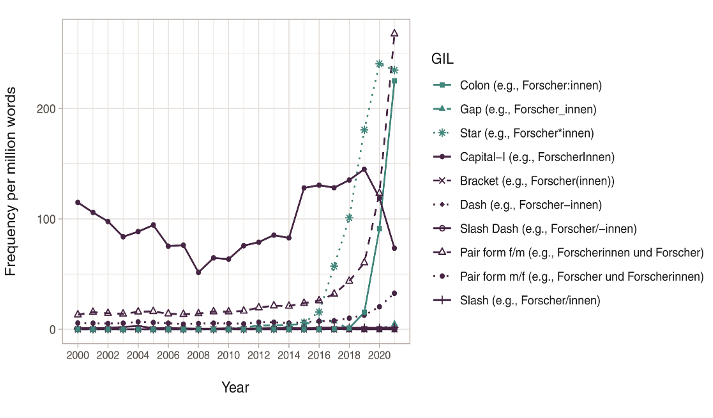
\includegraphics[width=1\textwidth]{gfl_types_frequency.png}
        \caption{Frequency of different types of gender-inclusive language. Source: \textcite{waldendorfWordsChangeIncrease2024} p. 367.}
        \label{fig:gfl_types_frequency}
    \end{figure}

    \subsubsection{Challenge of Integrating Gender-Fair Language into NLP}
    Although the use of GFL has increased in recent years \parencite{waldendorfWordsChangeIncrease2024}, it is still generally low. This leads to a scarcity of relevant linguistic data. Few datasets include GFL variants, and existing resources often depend on manual translations or post-editing to add gender-inclusive forms \parencite{lardelliBuildingBridgesDataset2024}. For this project, the limited availability of GFL data poses a significant challenge, especially when training the model to recognize gender-fair alternatives as neutral due to the lack of consistent examples.


    % --------------------------------------------------------------------------------

    \subsection{Research Gaps}
    A central gap in gender bias research is the absence of a shared definition of what constitutes "fair" language. This lack of conceptual clarity makes it difficult to design systematic evaluation approaches, define accountability standards, or detect all relevant forms of harm \parencite{barclayInvestigatingMarkersDrivers2024a,shresthaExploringGenderBiases2022,stanczakSurveyGenderBias2021}.

    A second major gap concerns the availability of high-quality EN-DE translation data that includes GFL. While a few datasets exist, they are not designed for bias detection tasks and often require manual post-editing to incorporate inclusive forms \parencite{lardelliBuildingBridgesDataset2024}. This limits the development and evaluation of models that aim to identify biased output in a structured and reproducible way.

    As \textcite{stanczakSurveyGenderBias2021} point out, findings on gender bias in English do not necessarily transfer to other languages such as German. This underlines the importance of typological diversity and language-specific solutions when addressing fairness in MT. Existing studies on EN-DE \parencite{ullmannGenderBiasMachine2022,kapplAreAllSpanish2025,lardelliBuildingBridgesDataset2024} systems mostly confirm the presence of gender bias, propose mitigation strategies, or introduce evaluation metrics. However, few provide methods for systematically detecting bias in translated text.

   This project addresses that gap by focusing on bias detection as a foundational step. To support this, I combine existing datasets from previous research to create a new dataset specifically for detecting gender bias in EN-DE translations. Given the lack of suitable data and tools, detection is a necessary starting point. Manual correction will likely remain necessary, as current research does not yet support reliable automatic debiasing. This project therefore focuses on flagging biased translations, not correcting them.

% --------------------------------------------------------------------------------

\section{Approach and Justification of the Technical Setup}
    This section outlines the technical setup used in the project and explains the rationale behind design choices. It also provides background information on the underlying technologies to clarify how each component contributes to the overall goal of detecting gender bias in EN-DE translations.

\subsection{Binary Classification in NLP}
    Binary classification means sorting items into two clear groups. It is the most common task in ML and is frequently found in every day life, such as automatically flitering e-mails as "spam" or "not spam" \parencite{quemyBinaryClassificationUnstructured2019} or deciding whether a transaction is "fraudulent" or "legitimate". For instance, a spam filter uses previously labeled e-mails to learn relevant patterns, such as specific keywords or sender information, and builds a model that applies these patterns to classify new messages accurately. 
    
    This thesis tries to label a translation as either "biased" or "neutral". While it is possible to extend the classification beyond two categories, such as distinguishing types of bias or including labels like "gender-fair", this would require much more data and training. Given the practical aim of this work, which is to help users quickly identify whether their text might contain gender bias, the model focuses on a simple binary decision.

\subsection{Transformer Architecture} \label{subsection:transformer_arch}
  To provide some background on the BERT architecture, it is important to understand its foundation in the Transformer model. The Transformer is designed to process input sequences and \textit{transform} them into output sequences. To do this effectively, it uses a self-attention mechanism \parencite{phuongFormalAlgorithmsTransformers2022}.

    \subsubsection{Self-attention mechanism}
    The self-attention mechanism allows the model to weigh the significance of all input elements simultaneously \parencite{xiaoIntroductionTransformersNLP2023}, meaning it can look at all words in a sentence at once and decide which ones are most relevant to each word. Unlike traditional methods like Recurrent Neural Networks (RNNs), which process input step by step, self-attention captures global dependencies and contextual relationships more accurately, creating "context-aware" representations.

    \subsubsection{Encoder-Decoder Framework} \label{subsection:encoder-decoder}
    The transformer architecture consists of two main components: the encoder and the decoder. The encoder’s job is to read the input sentence and turn it into a series of vectors the model can understand. Each vector is a list of numbers representing the meaning and structure of each word \parencite{xiaoIntroductionTransformersNLP2023}. The encoder works as follows (see \autoref{fig:transformer_architecture}):

    \begin{enumerate}
        \item It receives input embeddings, which represent the words, and positional encodings, which tell the model the order of the words.
        
        \item The data then passes through several identical layers. Each layer has two main parts:
        \begin{enumerate}[label=\alph*.]
            \item \textbf{Multi-head self-attention} runs several attention processes in parallel. Each attention head focuses on different details to help the model understand the sentence better.
            \item A \textbf{Feed-forward network} processes each word vector separately, refining the information like a small filter.
            \item \textbf{Add \& Layer Norm} combines a shortcut connection (Add) and normalization (Layer Norm). The Add step passes the original input forward to keep useful information. Layer Norm adjusts the output values to a stable range.
    \end{enumerate}
    
    \item Each layer builds on the output of the previous one, helping the model form more complex and abstract ideas about the input sentence.
    
    \item Finally, the encoder outputs a sequence of \textit{hidden states}. These are continuous vector representations for each input token. They encode contextual information from the entire sentence. For example, in the sentence "The cat sat on the mat," the vector for "cat" reflects its relationship to words like "sat" and "mat."
\end{enumerate}

\begin{figure}[ht]
    \centering
	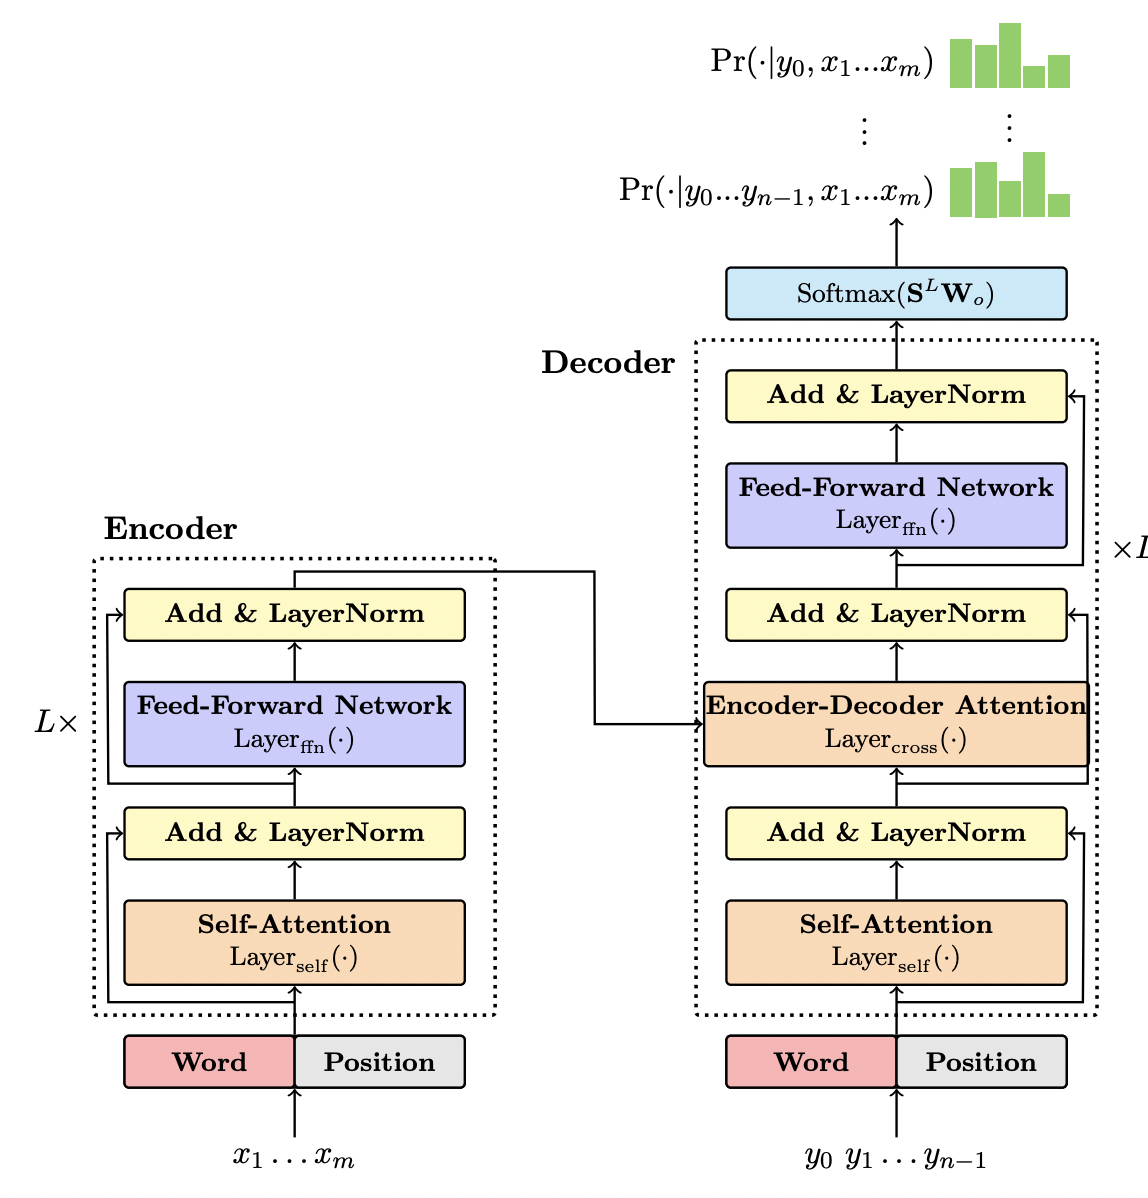
\includegraphics[width=\textwidth,height=0.45\textheight,keepaspectratio]{transformer_architecture.png}	
    \caption{Transformer encoder-decoder architecture. The encoder (left) processes input tokens \(x_1,\dots,x_m\) through: (1) a self-attention layer for contextual relationships, (2) a feed-forward network for feature transformation, and (3) residual connections with layer normalization. The decoder (right) generates outputs by attending to both the encoder's representations and its previous outputs ($y_0$ to $y_{n-1}$), producing the next-token probability distribution. Figure and description adapted from \textcite{xiaoIntroductionTransformersNLP2023}, p. 6.}
    \label{fig:transformer_architecture}
\end{figure}

The decoder generates the output sentence one word at a time by using the information from the encoder \parencite{xiaoIntroductionTransformersNLP2023}. However, since BERT uses only an encoder-only architecture (see \autoref{fig:bert_arch}), the decoder is not relevant for this work and is therefore excluded from the discussion.

\subsection{BERT}
    BERT is a language model that stands for "Bidirectional Encoder Representations from Transformers" and was introduced by Google in 2018 \parencite{devlinBERTPretrainingDeep2019}. After pre-training, BERT can be adapted to many NLP tasks by adding a simple output layer and fine-tuning, without needing major changes to its design. Since BERT uses only the encoder part of the Transformer architecture, it is designed to understand input rather than generate output. This makes it especially suitable for a binary classification task, where the goal is to analyze input texts and assign it to one of two categories.

    There are multiple variants of the original BERT model. It was originally released in two sizes: \texttt{BERT-Base} and \texttt{BERT-Large}, which differ in the number of layers, attention heads, and overall model capacity \parencite{devlinBERTPretrainingDeep2019}. Since then, many other versions have been developed. Most of them modify either BERT’s pre-training objectives or the underlying Transformer architecture \parencite{libovickyHowLanguageNeutralMultilingual2019}.

\subsection{Multilingual BERT (mBERT)}
    For this thesis, I use multilingual BERT \textbf{\href{https://huggingface.co/google-bert/bert-base-multilingual-cased}{(\texttt{mBERT})}} \parencite{devlinBERTPretrainingDeep2019}. \texttt{mBERT} uses the same configuration as \texttt{BERT-Base}, but it is pretrained on Wikipedia data from 104 languages, including both English and German. There is no explicit indication of the input language, nor is there a training objective that aligns languages bilingually. Instead, multilingual capabilities emerge naturally from its large multilingual text corpus \parencite{piresHowMultilingualMultilingual2019}.

    Monolingual models like \href{https://huggingface.co/google-bert/bert-base-german-cased}{\texttt{German BERT}} do not support English input. Larger multilingual models, such as \href{https://huggingface.co/docs/transformers/en/model_doc/xlm-roberta}{\texttt{XLM-RoBERTa}}, require more computational resources and training time, which was not feasible here. \texttt{mBERT} offers a good balance between language coverage, model size, and training efficiency, making it a practical choice detecting gender bias in EN-DE translations.

\begin{figure}
    \centering
	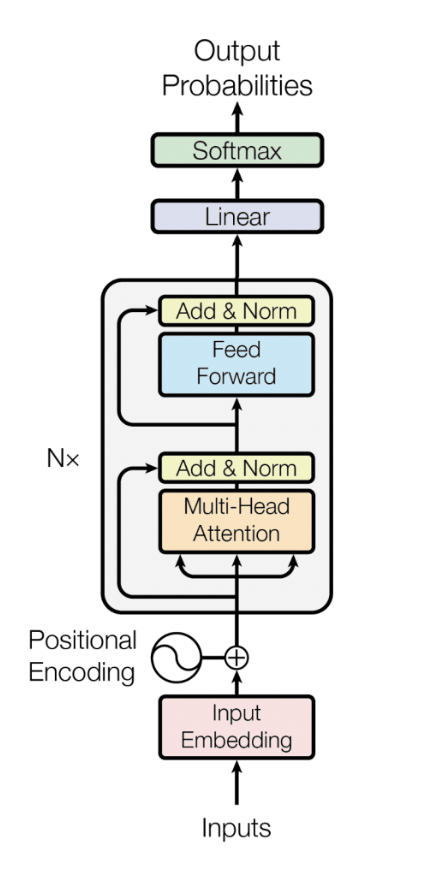
\includegraphics[width=\textwidth,height=0.4\textheight,keepaspectratio]{BERT_architecture.png}	
    \caption{BERT's encoder-only architecture. Figure by \textcite{smithCompleteGuideBERT2024}.}
    \label{fig:bert_arch}
\end{figure}

\subsubsection{Tokenization}
\texttt{mBERT} processes input by splitting words or subword units into \textit{tokens} (tokenization)\footnote{This tokenization process applies to both BERT and mBERT.}. It uses the WordPiece algorithm with a shared vocabulary of 110,000 tokens, and all texts are lowercased before tokenization \citep{devlinMultilingualBERTGitHub2018}. To balance the training data, languages with large Wikipedia corpora are downsampled, while those with fewer resources are oversampled.

Pre-processing is the same for all supported languages: (1) converting text to lowercase and removing accents, (2) splitting punctuation, and (3) tokenizing based on whitespace. Removing accents helps reduce the vocabulary size, even though it can introduce ambiguity in languages where accents carry meaning. This trade-off is accepted because \texttt{mBERT's} contextual embeddings usually resolve such ambiguities during training and inference.

Special tokens are reserved tokens added to in. They indicate boundaries or roles, helping the model distinguish parts of the text and process it correctly.

\begin{itemize}
	\item \texttt{[CLS]} (classification) marks the start of the sequence,
	\item \texttt{[SEP]} separates sentence pairs.
\end{itemize}

\noindent In this work, each input combines an English source sentence and its German translation as:

\begin{quote}
    \texttt{[CLS] english sentence [SEP] german translation [SEP]}
\end{quote}

\begin{quote}
\texttt{[CLS] the nurse is kind [SEP] die krankenschwester ist nett [SEP]}
\end{quote}

\subsubsection{Mechanics of Fine-Tuning mBERT}
    Fine-tuning adjusts the base model for a specific task, in this case, detecting gender bias in translations.\footnote{This fine-tuning process applies to both BERT and mBERT.} To do so, a new labeled dataset is used to continue training the model, allowing it to adapt its weights to task-specific patterns. 

    A classification head, comprising a linear layer followed by a softmax function (see \autoref{fig:bert_arch}), is added on top of \texttt{mBERT’s} output. The linear layer applies a learned transformation to the final hidden state vector of the \texttt{[CLS]} token. 

    \[
    z = Wx + b
    \]

    Here, \(x\) is the \texttt{[CLS]} embedding, \(W\) is the weight matrix, and \(b\) is the bias vector. Both \(W\) and \(b\) are parameters learned during training to help map \texttt{mBERT’s} output to the task labels. This changes the output into two numbers (logits), one for each class: biased or neutral. Then, the softmax function turns these numbers into probabilities \parencite{devlinBERTPretrainingDeep2019,xiaoIntroductionTransformersNLP2023}. Short for "soft maximum," it maps raw scores to a probability distribution, emphasizing the highest values while still giving smaller ones some weight.

    \[
    \text{softmax}(z_i) = \frac{e^{z_i}}{\sum_{j=1}^{K} e^{z_j}}
    \]

    Each logit \( z_i \) is exponentiated to ensure positivity. The result is then normalized by dividing by the sum of all exponentials, producing the probability distributions. \( K \) is the number of possible classes. The class with the highest probability is selected as the model’s prediction.
    
\subsubsection{Key Hyperparameters Explained}
    Fine-tuning can be unstable, and changes such as different seeds can lead to large differences in task performance \parencite{mosbachStabilityFinetuningBERT2021}. Tuning a set of key hyperparameters is therefore necessary. These are not learned by the model but must be set manually or through experimentation. Their values affect how fast the model learns, how stable training is, and how well the model generalizes to new data.

    The \textit{learning rate} controls how much the model updates its weights during each step \parencite{mosbachStabilityFinetuningBERT2021}. If it is too high, the model may not converge and instead jump over good solutions. If it is too low, training can be very slow or get stuck in local minima.

    \textit{Warmup steps} are used at the beginning of training to gradually increase the learning rate from zero to its target value \citep{mosbachStabilityFinetuningBERT2021}. This helps avoid instability in the early stages, where large updates can be harmful. After the warmup period, the learning rate is often decreased again using a scheduler, which controls how it changes over time.

    The \textit{number of epochs} defines how many times the model passes through the entire training dataset \parencite{mosbachStabilityFinetuningBERT2021}. More epochs mean more training iterations, which can help the model better fit the data. On small datasets, training for more epochs—sometimes up to 20 instead of the usual 3—helps reduce instability and improves generalization. This is because the model has more chances to learn meaningful patterns instead of stopping too early.

    The \textit{batch size} refers to how many training examples the model processes before updating its parameters \parencite{mosbachStabilityFinetuningBERT2021}. Commonly, a batch size of 16 is used during fine-tuning \texttt{mBERT}. Larger batches provide more stable gradient estimates but require more memory. Smaller batches can introduce noise in the updates but might help the model generalize better. While \textcite{mosbachStabilityFinetuningBERT2021} does not deeply analyze batch size effects on stability, it remains an important parameter to balance resource limits and training quality.

    Finally, the \textit{optimizer} controls how the model weights are adjusted to minimize prediction error \parencite{mosbachStabilityFinetuningBERT2021}. The AdamW optimizer is standard for \texttt{mBERT} fine-tuning because it adapts learning rates per parameter and includes weight decay regularization. A critical feature of Adam is \textit{bias correction}, which reduces the effective learning rate early in training. This acts like an implicit warmup, preventing large unstable updates and vanishing gradients in the lower layers. Combining explicit warmup with Adam’s bias correction allows training with higher learning rates more stably.

\subsection{Interactive Demo}
The fine-tuned model is intended to be presented through an interactive demonstration. Since the focus lies on showcasing the model’s functionality rather than creating a fully developed application, \href{https://streamlit.io/}{Streamlit} was chosen. Streamlit allows for quick and easy development of lightweight user interfaces in Python, providing a simple setup and effective performance. For live translation, an open-source tool supporting EN-DE pairs was required. \href{https://github.com/Helsinki-NLP/Opus-MT}{Opus-MT} \parencite{tiedemannOPUSMTBuildingOpen2020} meets these criteria and integrates smoothly into the demonstration. While state-of-the-art translators like Google Translate or DeepL would have been preferred for their quality, they do not meet the requirements for this setup. Therefore, a separate tab for manual translation input was added, allowing users to paste translations directly and bypass this limitation.
